\documentclass[times, 12pt]{article}
\usepackage{graphicx}
\author{Bogdan Carina\\
          Universitatea de Vest, Informatica aplicata}
 
 
\begin{document}         
\title {State of art pentru Echipa Sensor middleware}

\maketitle

\section{Senzor middleware}

Middleware este software-ul care ofer\u{a} o leg\u{a}tir\u{a} \^{i}ntre dou\u{a} aplica\c{t}ii soft diferite \c{s}i paseaz\u{a} datele \^{i}ntre ele. Middleware-ul ofer\u{a} posibilitatea de a  accesa datele aflate \^{i}ntr-o baz\u{a} de date s\u{a} fie accesate printr-o alta. Se mai poate spune c\u{a} middleware este software-ul de integrare de date.
ObjectWeb define\c{s}te middleware-ul ca fiind: "The software layer that lies between the operating system and applications on each side of a distributed computing system in a network."\footnote {Krakowiak, Sacha. "What's middleware?". } \^{I}n roman\u{a} :  "Stratul software care st\u{a} \^{i}ntre sistemul de operare \c{s}i aplica\c{t}ii \^{i}n fiecare parte a  sistemului distribuit a  re\c{t}elei. " 
Scopul priectului Sensor Middleware este de a  defini \c{s}i implementa o arhitectur\u{a} convenabil\u{a} care s\u{a} r\u{a}spund\u{a} cerin\c{t}elor impuse de construirea unei re\c{t}ele wireless de senzori care s\u{a} fie capabili s\u{a} detecteze, s\u{a} \^{i}nregistreze \c{s}i s\u{a} prelucreze date care vizez\u{a} m\u{a}rimi ale mediului cum ar fi: temperatura, curentul electric, consumul de gaz etc.

\section{Arhitectura minimal\u{a} }
Abordarea proiectului nostru va avea \^{i}n vedere trei probleme importante care constituie si nivelele arhitecturii modelului de snezor middleware:
\begin{enumerate} 
	\item Modelul hardware al senzorului	
\begin{itemize}
	\item construc\c{t}ia efectiv\u{a} tehnic\u{a} a  senzorilor
	\item topologia senzorilor adic\u{a} modelel arhitecturare de amplasare a  senzorilor \^{i}n cadrul locuin\c{t}ei
\end{itemize}
	\item Puntea \^{i}ntre hardware \c{s}i software
	\begin{itemize}
	\item dispozitivul de transformare a semnalelor analoage transmise de senzor \^{i}n semnale binare adic\u{a} date ce pot fi 	     \item prelucrate ulterior de un soft specializat
	\item stocarea datelor \^{i}ntr-o baza de date
\end{itemize}
	\item Modelul software de prelucrare a datelor care presupune
		\begin{itemize}
	\item agregarea datelor
	\item serializarea  datelor
	\item clusterizarea datelor
	\item generare de grafice
	\item compararea datelor
	\item detectarea punctelor de inflexiune
	\item detectarea erorilor cauzate de preluarea datelor
	\end{itemize}
\end{enumerate}

Abordarea middleware pentru re\c{t}ele de senzori a fost propus\u{a} pentru clusterizarea datelor, consumul de energie \c{s}i agregarea datelor \c{s}i a mecanismului de colectare  a acestora. Modelul midleware pentru Re\c{t}elele Wireless de Senzori \footnote{Wireless Sensor Network abreviat ca WSN} poate fi abordat din dou\u{a} puncte de vedere: abordarea bazat\u{a} pe baz\u{a} de date sau abordarea bazat\u{a} pe agent cea care satisface nevoile proiectului nostru.
Re\c{t}eaua de senzori este un sistem reactiv care va r\u{a}spunde schimbarilor de context bazate pe evenimente. Un agent este un cod special care se va plimba de-a lungul nodurilor \footnote{ Fiecare senzor care alc\u{a}tuie\c{t}te re\c{t}eaua de senzori va fi denumit generic nod } pentru a executa codul local pe baza evenimentului pe care il va primi. Modelul Sensor Ware \footnote { Boulis, C.C. Han, and M. B. Srivastava. Design and
�Implementation of a Framework for Programmable and Efficient
Sensor Networks�. In MobiSys 2003, San Francisco, USA, May
2003.} folose\c{s}te abordarea bazat\u{a} pe agen\c{t}i. \^{i}n acest model interpretorul de date ruleaz\u{a} pe fiecare nod care va detecta fiecare scimbare venit\u{a} din exterior. O alt\u{a} abordare bazat\u{a} pe modelula gent este Dfuse \footnote{ R. Kumar, M.Wolenetz, B. Agarwalla, J. Shin, P. Hutto,
A. Paul, and U. Ramachandran. DFuse:� A Framework
for Distributed Data Fusion�. SenSys, 2003.} care este similar\u{a} cu viziunile Sensor Ware. Aceste modele sunt implementate pe panouri embedded \^{i}n special pentru probleme cum ar fi snezorii de lumini\u{a} \c{s}i temperatur\u{a}.

\section{ Modele de construc\c{t}ie a senzorilor}

Vom prezenta c\^{a}teva modele de senzori de temperatur\u{a} care sunt deja dezvoltate \^{i}mpreun\u{a} cu avantajele \c{s}i dezavantajele pe care le prezint\u{a}. \^{i}n acest sens ne vom \^{i}ndrepta aten\c{t}ia spre senzorii de temperatur\u{a} din seria TE-6100.  Por\c{t}iunea senzitiv\u{a} a  acestor senzori este reprezentat\u{a} de elemente de nichel \c{s}i silicon a c\u{a}ror rezisten\c{t}\u{a} variaz\u{a} odat\u{a} cu schimbarea temperaturii. Modelele de senzori TE-6100 bazate pe fire de nichel sau tip de rezistent\u{a} bazate pe silicon confer\u{a} o rezisten\c{t}\u{a} variat\u{a} pentru un controller. C\^{a}nd temperatura senzorului se modific\u{a}, rezisten\c{t}a senzorului se modific\u{a} \^{i}n conformitate. Senzorul va ar\u{a}ta p schimbare pozitiv\u{a} de rezisten\c{t}\u{a} \^{i}n concorda\c{t}\u{a} cu temperatura. Senzorul de silicon se modific\u{a} $0.75\%$ per grad Celsius cu o referin\c{t}\u{a} la rezisten\c{t}\u{a} de 1035 ohms la 256 grade Celsius. Senzorul de nichel se modific\u{a} $5.4$ ohms per grad Celsius cu o referin\c{t}\u{a} la rezisten\c{t}\u{a} de $1000$ ohms la 21 grade Celsius. Modelele asem\u{a}n\u{a}toare dina ceast\u{a} categorie modelelor noastre de senzori sunt:
\subsection{Modelul TE-6100-1}
Acest model (figura de jos) este destinat pentru o palet\u{a} universal\u{a} de aplica\c{t}ii, \^{i}ns\u{a} acurate\c{t}ea \c{s}i consumul resurselor nu sunt prea avantajoase.


\begin{figure}
	\centering
		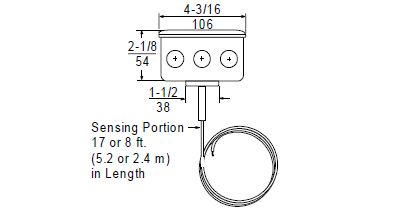
\includegraphics[height=60mm,width=70mm]{TE-1.JPG}
	\label{fig:TE-1}
\end{figure}


\subsection{Modelul  TE-6100-3}
Acest model (figura de jos) este destinat pentru controlul temperaturii \c{s}i memorarea acesteia. Modelul hardware include un element cu dou\u{a} cabluri de nichel, unul care s e intinde de-a lungul  a dou\u{a} cilindre concentrice \c{s}i altul care este izolat termic \c{s}i care este destinat producerii unu lag de timp la schimb\u{a}ri drastice de temperatur\u{a}.

{\bf \^{I}n modelul nostru}\\
\^{I}n modelul senzorului nostru schimb\u{a}rile drastice de temperatur\u{a} nu vor fi ignorate de hardware, ci \^{i}nregistrate ca date, iar ulterior \^{i}n procesul de prelucrare de date, pe baza unor marje de erori, vor fi excluse din calcul.


\begin{figure}
	\centering
		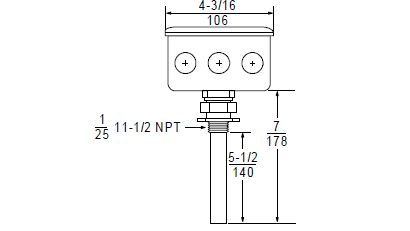
\includegraphics[height=60mm,width=70mm]{TE-2.JPG}
	\label{fig:TE-1}
\end{figure}

\section{Cerin\c{t}ele arhitecturii pentru re\c{t}elele de senzori}
\subsection*{Programabilitatea}
\^{i}n func\c{t}ie de tipul de senzor -sta\c{s}ionar sau mobil � re\c{t}eaua care faciliteaz\u{a} comunicarea \^{i}ntre senzorul fizic efectiv si ma\c{s}ina care va prelua datele trebuie s\u{a} \^{i}ndeplineasc\u{a} anumite cerin\c{t}e. Senzorii sta\c{t}ionari vor comunica prin protocoale preexistente si caracteristice tipului de  senzor ales, pe c\^{a}nd senzorii mobili vor avea  o re\c{t}ea de comunicare ad-hoc. Trebuie luat \^{i}n considerare \c{s}i pericolul de deconectare a senzorului de la re\c{t}ea, lungimea de band\u{a} mic\u{a}, limitarea aprovizion\u{a}rii cu energie a senzorilor, etc. \^{i}n conseciin\c{t}\u{a} re\c{t}eaua de senzori trebuie s\u{a} suporte func\c{t}ionalitate de programare, opera\c{t}ii asincrone \c{s}i o arhitectur\u{a} bazat\u{a} pe componente. Exist\u{a} asemenea  limbaje orientate eveniment care ar putea fi folosite pentru situa\c{t}iile \^{i}n care apar opera\c{t}ii de deconectare \c{s}i anume: NesC \footnote{ D. Gay, P. Levis, R. von Behren, M. Welsh, E. Brewer, and
D.Culler. �The nesC Language: A Holistic Approach to
Networked Embedded Systems�. In Proceedings of Programming
Language Design and Implementation (PLDI), June 2003.} \c{s}i galsC \footnote { Elaine Cheong, Jie Liu �galsC: A Language for Event-Driven
Embedded Systems� http://ptolemy.eecs.berkeley.edu}
 \^{I}ns\u{a} programarea fiec\u{a}rui senzor este dificil\u{a}, mai ales dac\u{a} exist\u{a} re\c{t}ele de senzori cu numeroase noduri. Noile paradigme de programare, asemenea celor abordate \^{i}n proiectul nostru, \^{i}\c{t}i \^{i}ndreapt\u{a} aten\c{t}ia spre func\c{t}ionalit\u{a}\c{t}i specifice la nivel de aplica\c{t}ie \c{s}i nu la nivel de nod. Solu\c{t}iile middleware eficiente pot ascunde complexitatea \^{i}n ceea ce prive\c{s}te configurarea individual\u{a} a nodurilor bazat\u{a} pe capabilit\u{a}\c{t}ile arhitecturii software \c{s}i hardware.

\subsection*{Adaptabilitatea}

Multe aplica\c{t}ii de senzori au nevoie s\u{a} i\c{s}i poat\u{a} schimba comportamentul \^{i}n func\c{t}ie de starea mediului \^{i}n care se afl\u{a}. De exemplu senzorii de lumin\u{a} vor trebui s\u{a} func\c{t}ioneze \^{i}n dou\u{a} moduri diferite \c{s}i anume \^{i}n regim de zi \c{s}i de noapte. Acest lucru este natural deoarece senzorii nu vor trebui s\u{a} detecteze lumina zilei ci doar acea lumin\u{a} venit\u{a} de la o surs\u{a} artificial\u{a}. \^{i}n caul \^{i}n care senzorul nu dispune de memorie suficient\u{a} pentru comutare de context, adic\u{a} de regim de func\c{t}ionare, atunci avem dou\u{a} posibilit\u{a}\c{t}i de a rezolva aceast\u{a} problem\u{a}. Prima ar fi c\u{a} datele vor trebui trimise unui server pentru lurea acestei decizii \c{s}i serverul va fi cel care va dicta senzorului regimul corespunz\u{a}tor de func\c{t}ionare. A doua op\c{t}iune ar fi ca senzorul s\u{a} aibe posibilitatea de a hot\u{a}r\^{i} singur ce regim s\u{a} urmeze urm\^{i}nd s\u{a} i\c{s}i downloadeze singur algoritmul necesar func\c{t}ion\u{a}rii care este disponibil pe serverul de decizie. Deoarece am convenit s\u{a} p\u{a}str\u{a}m luarea decizilor \c{s}i programarea la nivel de aplica\c{t}ie \c{s}i nu la nivel de nod proiectul nostru va aborda prima variant\u{a}. 

\subsection*{Scalabilitate}
Majoritatea implement\u{a}rilor de senzori profit\u{a} de localizarea spa\c{t}ial\u{a}. De exemplu, \^{i}n cazul senzorilor de detectare a misc\u{a}rii sau a temperaturii, informa\c{t}ia provenit\u{a} de la nodurile mai apropiate este evaluat\u{a} \c{s}i pe baza ei decizile ulteriaore vor fi f\u{a}cute. 

\subsection*{Dinamism mo\c{s}tenit}

Noduri noi ad\u{a}ugate \c{s}i eliminate din cuibul de senzori vor creea o schimbare \^{i}n topologia snezorilor. De aceea trebuie s\u{a} avem un mecanism pentru aplica\c{t}ie pentrua determina dinamic nodurile \c{s}i servicii suport.

\subsection*{Priorit\u{a}\c{t}i de timp real}
Re\c{t}elele de senzor sunt utilizate pentru amonitoriza fenomene de timp real \c{s}i nu alte informa\c{t}ii stocate. Acest lucru pune problema sign\u{a}rii priorit\u{a}\c{t}ilor \^{i}n timpul rul\u{a}rii \c{s}i cum s\u{a} men\c{t}inem ordinea natura\c{s}\u{a} de timp real. \^{i}n re\c{t}elele de senzori priorit\u{a}\c{t}iile trebuie s\u{a} fie explicit specificate. Prioritatea unui mesaj depinde de contexul sistemului. De aceea, priorit\u{a}\c{t}ile mesajelor trebui s\u{a} fie asignate la runtime de c\u{a}tre middleware \c{s}i ar trenui s\u{a} fie bazate pe context.
Managementul fuziunii senzorilor

Aplica\c{t}iile implicate \^{i}n detectarea misc\u{a}rii folosesc un num\u{a}r mare de senzori pentrua  identifica un obiect particular. Trebuie astfel \^{i}ntreprins un manager pentru fuziunea senzorilor care s\u{a} suporte fuziunea evenimentelor de nivel jos (cum ar fi temperatura mic\u{a} \c{s}i nivele de lumin\u{a}) pentru a prelucra evenimente de nivel \^{i}nalt cum ar fi detectarea obiectelor folosind diver\c{s}i algoritmi de fuziune.  Acest manager trebuie s\u{a} fie capabil s\u{a} selecteze rolul cel mai bun pentru modelele disponibile \c{s}i s\u{a} aloce roluri nodurilor din re\c{t}ea.

\subsection*{Manager de context}

Aplica\c{t}iile cu senzori necesit\u{a} adapt\u{a}ri \^{i}n func\c{t}ie de schimb\u{a}rile comportamentului \c{s}i trebuie s\u{a} se poat\u{a} adapta la un context anume \^{i}n care trebuie s\u{a} lucreze. Contextul poate fi definit ca un set de st\u{a}ri de schimbare care vor conduce la o stare particular\u{a} a re\c{t}elei.

\section{Achizi\c{t}ionarea datelor de la senzor}

Achizi\c{t}ionarea datelor este procesul de acumularea  semnalelor care m\u{a}soar\u{a} condi\c{t}ii fizice din lumea real\u{a} \c{s}i de conversie a reultatelor preluate \^{i}n valori digitale numerice care ulterior pot fi manipulate de calculator. Sistemele de achizi\c{t}ie a  datelor de la senzori(abreviate DAS sau DAQ), \^{i}n mod tipic, convertesc forme ondulatorii analogice \^{i}n valori digitale menite prelucr\u{a}rii computerizate. Componentele unui astfel de sistem sunt:
\begin{itemize}
	\item Senzorii care convertesc parametrii fizici \^{i}n semnale electrice
	\item Circuite de condi\c{t}ion\u{a}ri ale semnalelor pentru convertirea semnalelor de la sezori \^{i}ntr-o form\u{a} care va putea  fi convertit\u{a} \^{i}n valori digitale.
	\item Convertoare analog spre digital, care vor converti semnalele senzorilor \^{i}n valori digitale
\end{itemize}
Aplica\c{t}iile de achizi\c{t}ie de date sunt controlate de programe soft dezvoltate folosind limbaje de programare diferite, \^{i}n cazul nostru Java. Pentru a accesa si controla data preluat\u{a} de hardware-ul de achizi\c{t}ionare se va putea folosi un API care va putea rula pe diverse sisteme de operare.

Achizi\c{t}ionarea datelor va \^{i}ncepe cu fenomenul fizic sau proprietatea fizic\u{a} care urmeaz\u{a} a fi m\u{a}surat\u{a}, cum ar fi temperatura, intensitatea luminii, consumul de energie electric\u{a}, consumul de gaz etc. Indiferent de m\u{a}rimea  fizic\u{a} m\u{a}surat\u{a}, starea fizic\u{a} care urmeaz\u{a} a fi m\u{a}surat\u{a} trebuie s\u{a} fie mai \^{i}nt\^{a} transformat\u{a} \^{i}ntr-o form\u{a} unic\u{a} care va putea  fi preluat\u{a} de sistemul de achizi\c{t}ie. Aceast\u{a} transformare va fi rea\c{s}izat\u{a} de snezorul efectiv.

Abilitatea de receptare de date a sistemului depinde de tipul de senzor care va detecta varia\c{t}ia propriet\u{a}\c{t}ii fizice respective. DAQ necesit\u{a} numeroase tehnici de condi\c{t}ionare pentru semnalempentru a modifica numeroase semnale electrice  \^{i}n curent electric pentru a fi digitalizate utiliz\^{a}nd Convertorul analog spre digital ( Analog-to-digital converter (ADC) ).

Semnalele pot fi digitale, numile semnale logice, sau analoage. Condi\c{t}ionarea semnalelor ar putea  fi necesar\u{a} dac\u{a} semnalele preluate nu sunt inteligibile pentru hardware-ul DAQ utilizat. Semnalul va trebui fie amplificat, filtrat, fie demodulat.\\


{\bf Conversia analog spre digital}\\


Un convertor analog la digital (analog-to-digital converter ADC) este un dispozitiv care va converti o cantitate continu\u{a} la un num\u{a}r digital discret. Tipic ADC-ul este un dispozitiv electronic care va converti un input analog de un anumit voltaj sau curent \^{i}ntr-un num\u{a}r digital propor\c{t}ional cu magnitudinea care define\c{s}te curentul sau voltajul. Output-ul digital folose\c{s}te o numeroase scheme de codificare diferite. Un ADC poate fi folosit s\u{a} m\u{a}soare valori izolate, \^{i}ns\u{a} \^{i}n cazul nostru se vor folosi semnale dependente de timp \c{s}i le va transforma \^{i}n secven\c{t}e digitale. Rezultatul va fi o cantitate de date m\u{a}surat\u{a} at\^{a}t \^{i}n timp, c\^{a}t \c{s}i \^{i}n valoare.
Semnalele pot fi \^{i}ncadrate \^{i}n numeroase categorii, \^{i}ns\u{a} distinc\c{t}ia cea  mai comun\u{a} se realizeaz\u{a} \^{i}ntre semnalele discrete \c{s}i cele continue \^{i}n func\c{t}ie de func\c{t}iile matematice peste care sunt definite. Semnale discrete de timp sunt deseori referite ca \c{s}i serii de timp. Semnalele continue de timp sunt referite ca simplu semnale continue. 

Un semnal discret sau un semnal discret de timp este o serie de timp care reprezint\u{a} o secven\c{t}\u{a} de anumite cantit\u{a}\c{t}i. Cu alte cuvinte, reprezint\u{a} o serie de timp care este o func\c{t}ie definit\u{a} peste un domeniu de numere discrete. Fiecare valoare a secven\c{t}ei s e nume\c{s}te e\c{s}antion sau prob\u{a}.
Spre deosebire de semnalele continue, un semnal discret nu este o fun\c{t}ie de un argument continuu, chiar dac\u{a} se poate ca semnalul s\u{a} fi fost ob\c{t}inut prin colectarea unui smenal continuu. Atunci c\^{a}nd un semnal discret corespunde unor valori uniforme de timp, va exista o rat\u{a} de colectare. Rata de colectare nu va fi prezent\u{a} \^{i}n secven\c{t}a de date, deci va trebui s\u{a}  s e  atribuie o variabil\u{a} separat\u{a}.\\

Semnalul digital utilizat va fi un semnal dintr-o serie discret\u{a} de timp pentru care amplitudine a si timpul sunt discrete \c{s}i care va lua un singur ste de valori discrete \c{s}i de asemene a input-ul \c{s}i output-ul sunt discrete.

\begin{figure}
	\centering
		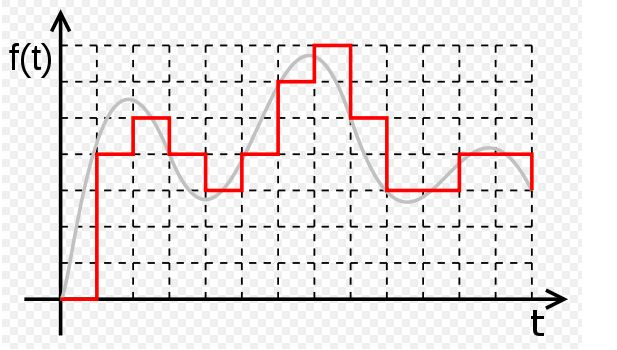
\includegraphics[height=50mm,width=50mm]{p1.JPG}
	\label{fig:p1}
\end{figure}

\begin{figure}
	\centering
		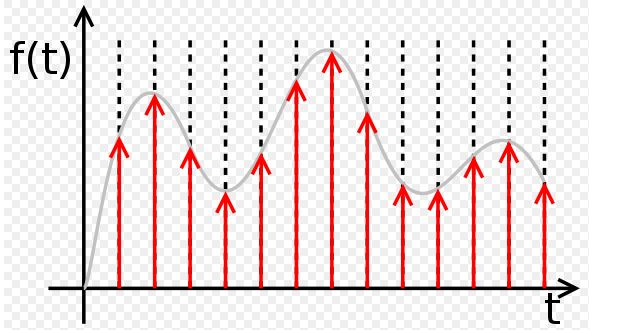
\includegraphics[height=50mm,width=50mm]{p2.JPG}
	\label{fig:p1}
\end{figure}


Seria de date utilizat\u{a} va fi o secven\c{t}\u{a} de puncte de date, m\u{a}surate la valori de timp succesive \c{s}i uniforme. Intervalul nostru de timp \^{i}ntre m\u{a}sur\u{a}tori va fi constant de 6 secunde. 

Serile de date au o ordine temporal\u{a} natural\u{a}. Acest lucru le afce distincte de alte probleme de analiz\u{a} a  datelor \^{i}n care nu exist\u{a} o ordine natural\u{a} a observ\u{a}rilor. Un model de serii de date va reflecta \^{i}n general faptul c\u{a} observ\u{a}rile apropiate ca timp vor fi \c{s}i mai apropiate dec\^{a}t observ\u{a}rile realizate \^{i}ntr-un timp viitor. \c{s}i mai mult, modelele serilor de date vor face uz de ordonarea \^{i}ntr-o singur\u{a} direc\c{t}ie astfel \^{i}nc\^{a}t valorile pentru o perioad\u{a} dat\u{a} de timp va fi exprimat\u{a} ca fiind derivat\u{a} din valori din trecut \c{s}i nu valori din viitor.

\section{ Prelucr\u{a}ri software ale serilor de date}
\subsection{Clusterizarea datelor provenite de la senzori}

Analiza bazat\u{a} pe clusterizare este procedeul de a  g\u{a}si grupuri de similarit\u{a}\c{t}i \^{i}ntr-o serie de date. Deoarece evenimentele vizate pentru prelucarre sunt prea individuale, ele vor fi grupate \^{i}n anumite grupuri bazate pe anumite tr\u{a}s\u{a}turi similare. Un termen necesar aici este {\it clasificarea} procesul de asignare a unui nou item sau observa\c{t}ie la locul s\u{a}u potrivit \^{i}ntr-un set predefinit de clase de categorii.

Clusterizarea serilor de date cu variabile multiple are ca scop gruparea seturilor de date care au caracteristici similare. Aceste grupuri pot fi analizate ulterior \^{i}n detaliu pentru a face descoperiri \^{i}n miezul caracteristicilor comune a fiec\u{a}rui grup de date. \\

{\bf Clusterizarea folosind factori de similaritate}\\

Factorii de similaritate pot fi folosi\c{t}i \^{i}n locul distan\c{t}ei Euclidiene(abordare veche) pentru a  m\u{a}sura similaritatea \^{i}ntre dou\u{a} seturi de date multivariate $X{_1}$ \c{s}i $X_{2}$. Krzanowski \footnote{ Oxford Statistical Science Books, W. Krzanowski, Principle of Multivariate Analisys} a dezvoltat o metod\u{a} pentru m\u{a}surarea similarit\u{a}\c{t}ii a dou\u{a} seturi de date folosind factorul de  similaritate PCA care se va calcula folosind componenta $ k$ cea  mai mare a  fiec\u{a}rui set de date. Componentele principale (PC) sunt vectorii matricei de covarian\c{t}\u{a} a setului de date multivalori. Factorul de similaritate $S_{PCA}$ este definit ca :
	\[S_{PCA}=^{\Delta}\frac{1}{k}\sum^{k}_{i=1}\sum^{k}_{j=1}cos^{2}\theta_{ij}
\]
unde $k$ este num\u{a}rul selectat din ambele seturi de date, $\theta_{ij}$ este unghiul dintre al i-lea PC a lui $X_{1}$ \c{s}i al j-mea PC alui $X_{2}$. Num\u{a}rul de PC-uri, $k$, poate fi ales astfel \^{i}nc\^{a}t PC-ul k s\u{a} descrie cel pu\c{t}in $95\%$ varian\c{t}\u{a} \^{i}n fiecare set de date.\\

{\bf Algoritmul propus este cel care folose\c{s}te K mijloace de factori de similaritate}\\

Fiind date $Q$ seturi de date, ${X_{1},...,X_{q},...,X_{Q}}$, trebuie s\u{a} fie clusterizate(\^{i}ncuibate ) \^{i}n K clustere.
\begin{enumerate}
	\item Fie al j-lea set de date reprezentat \^{i}n al i-lea set de date numit $X^{(i)}_{j}$. Se va computa setul de date agregat $X_{i}(i=1,...,K)$, pentru fiecare din cele K clustere ca fiind:
	\[X_{i}=[(X^{(i)}_{1})^{T}...(X^{(i)}_{j})^{T}...(X^{(i)}_{Q_{i}})^{T}]^{T}
\]
unde $Q_{i}$ este num\u{a}rul de seturi de date \^{i}n $X_{i}$. S\u{a} se  consemneze c\u{a} $\sum^{K}_{i=1}Q_{i=Q}$.
\item Se va calcula disimilaritatea \^{i}ntre setul de date $X_{q}$ \c{s}i fiecare din cele K clustere agregate $X_{i},i=1,...,K$ ca fiind:
	\[d_{i,q}=1-SF_{i,q}
\]
unde $SF_{i,q}$ este factorul de similaritate \^{i}ntre al q-lea set de date \c{s}i al i-lea cluster. Apoi se  va l\u{a}sa setul de date agregat $X_{i}$ s\u{a} fie setul de date de referin\c{t}\u{a}. Setul de date $X_{q}$ va fi asignat cluster-ului c\u{a}ruia \^{i}i este cel mai pu\c{t}in nesimilar \c{s}i anume clusterul cu valoarea cea  mai mic\u{a} a lui $d_{i,q}$. Se va repeta pasul pentru toate Q clustere.
\item Se va calcula media nesimilarit\u{a}\c{t}ilor a  fiec\u{a}rui set de date dup\u{a} formula:
	\[J(K)=\frac{1}{Q}\sum^{K}_{i=1}\sum^{}_{X_{q}\in X_{i}}d_{i,q}
\]
\item Dac\u{a} valoarea lui $J(K)$ s-a schimbat dinaintea primei itera\c{t}ii atunci ne vom \^{i}ntoarce la pasul 2, altfel stop.
\end{enumerate}

\subsection{ Compararea seriilor de date pentru sisteme de senzori }
\^{I}n statistici , corela\c{t}ia \c{s}i dependen\c{t}a sunt elemente dintr-o clas\u{a} larg\u{a} de rela\c{t}ii statistice \^{i}ntre dou\u{a} sau mai multe variabile aleatoare sau de date, de valori observate. Exist\u{a} dou\u{a} metode de comparare a serilor de date dup\u{a} cu urmeaz\u{a}:
M\u{a}sura cea mai cunoscut\u{a} de dependen\c{t}\u{a} \^{i}ntre dou\u{a} cantit\u{a}\c{t}i este coeficientul Pearson sau "de corela\c{t}ie Pearson� . Acesta se ob\c{t}ine prin \^{i}mp\u{a}r\c{t}irea covariant\u{a} dintre cele dou\u{a} variabile la produsul abaterilor standard .
Coeficientul de corela\c{t}ie a popula\c{t}iei $\rho,X,Y$ dintre dou\u{a} variabile aleatoare $X$ \c{s}i $Y$ cu valorile a\c{s}teptate $\mu\mu X$ \c{s}i $Y$ \c{s}i abaterile standard $\sigma X$ \c{s}i $\sigma Y$, este definit astfel: 
	\[\rho_{X,Y}=corr(X,Y)=\frac{cov(X,Y)}{\rho_{X}\rho_{Y}}=\frac{E[(X-\mu_{X})(Y-\mu_{Y})]}{\rho_{X}\rho_{Y}}
\]
unde E este valoarea a\c{s}teptat\u{a}, cov \^{i}nseamn\u{a} covarian\c{t}\u{a} \c{s}i corr fiind o nota\c{t}ie alternativ\u{a} utilizat\u{a} pe scar\u{a} larg\u{a} pentru corela\c{t}ie Pearson. 
Corela\c{t}ia Pearson este definit\u{a} numai dac\u{a} ambele devia\c{t}ii standard sunt finite \c{s}i ambele dintre ele sunt nenule. Este un corolar al inegalit\u{a}\c{t}ii Cauchy-Schwarz deoarece aceast\u{a} corela\c{t}ie nu poate dep\u{a}\c{s}i 1 \^{i}n valoare absolut\u{a} . Coeficientul de corela\c{t}ie este simetric: $Corr (X, Y) = Corr (Y, X)$. 

Corela\c{t}ia Pearson este 1 \^{i}n cazul unei rela\c{t}ii liniare perfecte pozitive (\^{i}n cre\c{s}tere), -1 \^{i}n cazul unei rela\c{t}ii liniare perfecte negative (de scadere) \c{s}i are valori cuprinse \^{i}ntre -1 \c{s}i 1 \^{i}n toate celelalte cazuri care indic\u{a} gradul de dependen\c{t}\u{a} liniar\u{a} \^{i}ntre variabile. Cu cat coeficientul este mai aproape de a fi -1 sau 1, cu at\^{a}t mai puternic\u{a} este corela\c{t}ia dintre variabile.  \\

{\bf Coeficientul Pearson utilizat \^{i}n compararea seriilor de date pentru sisteme de senzori }\\

Fiind date serii de timp care reprezint\u{a} consumul de curent electric se dore\c{s}te o comparare low-end a utilizatorilor sau respectiv a claselor de utilizatori. Pentru aceasta ne putem folosi de coeficientul Pearson de dependen\c{t}\u{a} liniar\u{a} ( deoarece graficele de consum sunt compuneri de func\c{t}ii liniare ). 
Pentru a aplica coeficientul Pearson asupra unor seturi de date, acestea trebuie \^{i}nt\^{a}i normalizate. 

Prin normalizarea seturilor de date se \^{i}n\c{t}elege: 
\begin{enumerate}
\item Ambele seturi s\u{a} aib\u{a} acela\c{s}i num\u{a}r de elemente 
\item Ambele seturi s\u{a} fie reprezentate pe aceea\c{s}i scar\u{a}
\item Eliminarea �Zgomotului�
\end{enumerate}

{\bf Algoritmul pentru generarea coeficientului Pearson}

\begin{enumerate}
	\item Vom avea \^{i}n vedere dou\u{a} seturi de date $S_{1}$ \c{s}i $S_{2}$, abaterile standard a celor dou\u{a} seturi $d_{x}$ \c{s}i $d_{y}$ \c{s}i medile aritmetice $m_{1}$ si $m_{2}$ ale valorilor fiec\u{a}rui set de date 
se va calcula abaterea standard a setului 1 de date apoi a setului 2 de date conform formulei:

	\[\sigma=\sqrt{\frac{1}{N}\sum^{i=1}_{N}(x_{i}-\mu)^{2}}
\]
unde $\sigma$ este abaterea standard, N este m\u{a}rimea setului de valori, $x_{i}$ este valoarea considerat\u{a}, $\mu$ este media valorilor setului.
	\item Apoi se va calcula media aritmetic\u{a} a tuturor valorilor setului 1  de date, respectiv setul 2 de date
vom lua ca iterator o variabil\u{a} i care va \^{i}ncepe la 0 \c{s}i se va incrementa cu o unitate c\^{a}t timp variabila i va fi mai mic\u{a} dec\^{a}t num\u{a}rul de valori din setul de date
la fiecare pas se va calcula raportul dintre diferen\c{t}a dintre valoarea extras\u{a} din set \c{s}i media setului respectiv \c{s}i devia\c{t}ia standard  a setului. Acest procedeu se va repeta pentru fiecare set. La fiecare pas vom avea  o variabil\u{a} rezultat care va p\u{a}stra radicalul produsului opera\c{t}iei calculate pentru setul 1 respectiv setul 2.
	\item La sf\^{a}r\c{s}it se va face \^{i}mp\u{a}r\c{t}irea unit\u{a}\c{t}ii la prodului sumei rezultatelor de la fiecare pas cu m\u{a}rimea setului \^{i}n cauz\u{a}.
\end{enumerate}

A doua metod\u{a} se nume\c{s}te {\bf Circle Matching}\\

Circle matching se bazeaz\u{a} pe algoritmi primitivi de comparare de imagini. 

Algoritmul utilizat prime\c{s}te ca date de intrare 2 grafice de consum ce reprezint\u{a} seturile de date de comparat \c{s}i returneaz\u{a} o valoare \^{i}ntre 0 si 100 ce reprezint\u{a} procentajul de similaritate. 
Algoritmul func\c{t}ioneaz\u{a} pe urm\u{a}toarele principii: 

Fie graficul de consum A � ro\c{s}u \c{s}i graficul de consum B � albastru 
Circle matching va detecta pentru fiecare punct al graficului A- puncte albastre \^{i}n proximitatea sa (proximitate determinat\u{a} de o constant\u{a} alfa, aleas\u{a} \^{i}n func\c{t}ie de m\u{a}rimea setului de date ) 

Fiecare punct ce indepline\c{s}te condi\c{t}ia de proximitate incrementeaz\u{a} un contor; 
Algoritmul returneaz\u{a} valoarea: {\it Contor/Num\u{a}rTotalPuncte(A+B)}

\subsection{ Detectarea anomaliilor din fluxul de date a senyorilor de mediu}

Unii senzori opereaz\u{a} \^{i}n condi\c{t}ii grele, iar datele trimise de ace\c{s}tia c\u{a}tre re\c{t}elele de comunicare, pot deveni eronate. Senzorii insitu sunt acei senzori care sunt localizati \^{i}n mediul \^{i}n care monitorizeaza.
Tipurile de erori pot fi cauyate chiar de ace\c{s}tia, de transmiterea unor date eronate, sau de comportamentul ocazional al sistemului, lucruri care sunt de interes pentru comunit\u{a}\c{t}iile de \c{s}tiin\c{t}\u{a}. A\c{s}adar avem nevoie de o asigurare \c{s}i un control \^{i}n mod automat a calit\u{a}\c{t}ii datelor(QA/QC). Acest lucru este foarte util atunci c\^{a}nd dorim s\u{a} facem o analiz\u{a} mai detaliat\u{a} a datelor, care la prima vedere pot p\u{a}rea anormale sau pentru care trebuie s\u{a} executam cu totul alte ac\c{t}iuni(de exemplu cazul unui dezastru natural). Aplica\c{t}ia cere ca datele anormale s\u{a} fie verificate \^{i}n timp aproape real, deci trebuie s\u{a} fie rapid \c{s}i efectuat incremental pentru a putea \c{t}ine pasul cu rata colect\u{a}rii de date. 

Pentru aceast\u{a} metod\u{a}, se propune un senzor de simulare, ale c\u{a}rui m\u{a}sur\u{a}tori vor fi comparate cu m\u{a}sur\u{a}torile senzorului actual. Astfel, vom clasifica o dat\u{a} ca fiind normal\u{a} sau anormal\u{a} pe baza diferen\c{t}ei dintre anticip\u{a}rile modelului \c{s}i m\u{a}sur\u{a}toarea senzorului. Acest studiu dezvolt\u{a} o metod\u{a} de detec\c{t}ie a anomaliilor \^{i}n timp real, care angajeaz\u{a} un model de data-driven unidimensional a fluxului de date \c{s}i un interval de predic\c{t}ie (PI), calculat dintr-un istoric recent. 

Datele vor fi clasificate ca fiind normale \^{i}n func\c{t}ie de aser\c{t}iunea c\u{a} rezultatul va fi PI sau nu. Aceast\u{a} metod\u{a} nu cere niciun exemplu preclasificat de date, ci se potriveste unui volum larg de date \c{s}i permite o evaluare de date incremental\u{a} rapid\u{a}, din momentul \^{i}n care devine disponibil\u{a}.\\

{\bf Algoritmul pentru detectarea anomaliilor din serile de date}\\

Acest studiu propune o metod\u{a} de redundan\c{t}\u{a} analitic\u{a} pentru detectarea anomaliilor, care folose\c{s}te o fereastr\u{a} mobil\u{a} de q m\u{a}sur\u{a}tori ale senzorilor (sau valorile pe care le a\c{s}tept\u{a}m de la ace\c{s}tia): 
	\[D^{t}={x_{t-q+1},...,x_{t}}
\]

pentru a clasifica urm\u{a}toarele secven\c{t}e de m\u{a}sur\u{a}tori. M\u{a}sur\u{a}toarea va fi clasificat\u{a} ca fiind anormal\u{a} dac\u{a} deviaz\u{a} semnificativ de la valoarea anticipat\u{a} f\u{a}cut\u{a} cu un pas \^{i}nainte. Apoi metoda umple geamul cu q-ul cel mai recent \c{s}i se continu\u{a} clasificarea cu urm\u{a}toarea m\u{a}sur\u{a}toare primit\u{a} de la senzor. Avem urm\u{a}torii pa\c{s}i \^{i}ncep\^{a}nd de la timpul t:

\^{I}naintea valorilor calculate folosind $D^{t}$ ca dat\u{a} de intrare.
Apoi metoda umple geamul cu q-ul cel mai recent \c{s}i se continu\u{a} clasificarea cu
urmatoarea m\u{a}suratoare luat\u{a} de la senzor. Avem urmatorii pa\c{s}i (\^{i}ncep\^{a}nd de
la timpul $t$):
\begin{enumerate}
	\item Metoda de anticipare cu un pas \^{i}nainte ia ca input $D^{t}$ pentru a anticipa $x_{t+1}$ valoare a\c{s}teptat\u{a} de la senzorul m\u{a}surat la timpul $t+1$;
	\item Calculeaz\u{a} leg\u{a}turile din intervalul de anticipare cu probabilitatea $p$, realiz\^{a}nd un rang
	\item Compar\u{a}m m\u{a}surarea de la timpul $t+1$ cu (2) . Dac\u{a} datele nu apar\c{t}in
intervalului rangului de la (2) atunci sunt considerate ca fiind anormale.
	\item(a) Sub strategia de detec\c{t}ie a anomaliilor si a atenu\u{a}rii (ADAM), daca
m\u{a}suratoarea este clasificat\u{a} ca fiind anormal\u{a} modific\u{a} $D^{t}$ \c{s}terg\^{a}nd $x_{t-q+1}$ din  spatele ferestrei \c{s}i ad\u{a}ug\^{a}nd $x_{t+1}$ \^{i}n fa\c{t}a ferestrei pentru a crea $D^{t+1}$ 
	\item(b)Daca m\u{a}sur\u{a}toarea este clasificat\u{a} ca fiind normal\u{a}, modific\u{a} $D^{t}$ sterg\^{a}nd $x_{t-q+1}$ din spatele ferestrei \c{s}�i ad\u{a}ug\^{a}nd $x_{t+1}$ \^{i}n fa\c{t}a ferestrei pentru a crea $D^{t+1}$.
\item repeta pa\c{s}ii 1-4.
\end{enumerate}

\begin{figure}
	\centering
		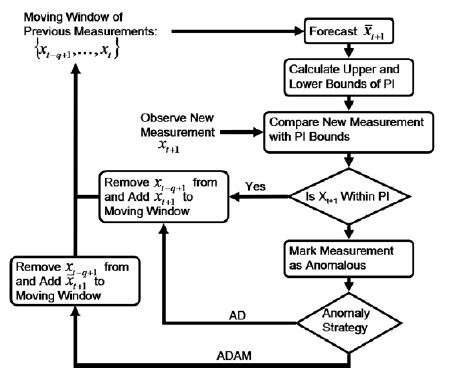
\includegraphics[height=60mm,width=60mm]{p4.JPG}
	\label{fig:p4}
\end{figure}

\subsection{ Num\u{a}rarea elementelor distincte dintr-un flux de date }

\^{I}n bazele de date, o problem\u{a} fundamental\u{a} o reprezint\u{a} num\u{a}rarea elementelor
diferite dintr-un tabel.
Avem nevoie de un algoritm de optimizare a datelor primite \^{i}ntr-un anumit
timp \c{s}i spa\c{t}iu. Acest algoritm este considerat eficient dac\u{a} folose\c{s}te foarte pu\c{t}in spa\c{t}iu, dac\u{a} are unul sau c\^{a}t mai pu\c{t}ine cicluri \c{s}i dac\u{a} proceseaz\u{a} fiecare element introdus \^{i}ntr-un timp c\^{a}t mai scurt.
Presupunem c\u{a} avem un \c{s}ir de elemente $a_{1},...a_{n}$, $n$ apar\c{t}ine domeniului $|m|={1,...,m}$.
$F_{0}=F_{0}(a)$(cu alte cuvinte momentul frecven\c{t}ei 0) reprezint\u{a} num\u{a}rul elementelor distincte care apar \^{i}n secven\c{t}\u{a}. Algoritmul care aproximeaz\u{a} $F_{0}$ este considerat eficietn dac\u{a} folose\c{s}te mai mul\c{t}i $(1/\epsilon,log n,log m)$ bi\c{t}i de memorie, unde $1\pm\epsilon$ este un factor \^{i}n cadrul c\u{a}ruia $F_{0}$ trebuie s\u{a} fie aproximat.

Vom prezenta trei algoritmi cu diferite echilibr\u{a}ri timp-spa\c{t}iu pentru aproximarea lui $F_{0}$. Algoritmii vor fi condi\c{t}iona\c{t}i de $\epsilon$ si $log m$(surprim\^{a}nd dependen\c{t}a de n). de exemplu dac\u{a} $m<n$ este mult mai avantajos s\u{a} avem algoritmi ai c\u{a}ror leg\u{a}turi depind de $log m$ \c{s}i nu de $log n$, iar dac\u{a} $m>n$ putem realiza un mic truc utiliz\^{a}nd o dispersie a datelor, care reduce descrierea fiec\u{a}rui element \^{i}n curs $(O(logn))$. De asemenea presupunem c\u{a} exist\u{a} $\epsilon_{0}<1$ \^{i}n a\c{s}a fel \^{i}nc\^{a}t acurate\c{t}ea parametrului $\epsilon$ dat algoritmului este cel mult $\epsilon_{0}$. \\

\begin{figure}
	\centering
		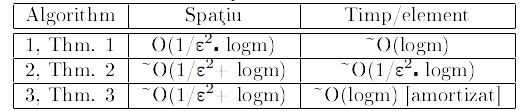
\includegraphics[height=25mm,width=110mm]{p5.JPG}
	\label{fig:p5}
\end{figure}


{\bf Algoritmul 1}\\
Acest algoritm alege la \^{i}nt\^{a}mpalre o func\c{t}ie $h:|m|->[0,1]$. Apoi aplic\u{a} func\c{t}ia la fiecare element din a \c{s}i men\c{t}ine valoarea $v=min^{n}_{j}h(a_{j})$. \^{I}n final estimarea va fi $F_{0}=1/v$.
Apoi, mai lu\u{a}m o func\c{t}ie $h:|m|->[0,1]$, dar men\c{t}inem elementele $a_{i}$ la $t=O(1/\epsilon^{2})$ pe care func\c{t}ia h le va evalua la cea mai mic\u{a} valoare t.
Estimarea $F_{0}=1/v$. , v fiind valoarea t cea mai mic\u{a}.\\

{\bf Teorema 1 }
Avem un algoritm care pentru oricare $\epsilon$, $\delta>0$,$(\epsilon,\delta)$ aproximeaz\u{a} $F_{0}$ folosind $O(1/\epsilon^{2}*log m*log(1/\delta))$ bi\c{t}i de memorie \c{s}i $O(1/\epsilon^{2}*log m*log(1/\delta))$ timp de procesare per element. \\
{\it Demonstra\c{t}ie:}
Lu\u{a}m o pereche independent\u{a} de func\c{t}ie $h>|m|->|M|$, unde $M=m^{3}$ este injectiv\u{a} pe elementele lui a. Cu probabilitatea cel pu\c{t}in $1-1/m$.\\

{\bf Algoritmul 2 }
Scopul acestui algoritm este s\u{a} defineasc\u{a} o cantitate care poate fi aproximat\u{a} \^{i}ntr-un model de flux de date \c{s}i care poate fi folositp pentru aproximarea lui $F_{0}$.\\

{\bf Teorema 2}
Avem un algoritm care pentru  oricare $\epsilon$, $\delta>0$,$(\epsilon,\delta)$ aproximeaz\u{a} $F_{0}$ folosind $O(1/\epsilon^{2}*log m*log(1/\delta))$ bi\c{t}i de memorie \c{s}i $O(1/\epsilon^{2}*log m*log(1/\delta))$ timp de procesare per element.

{\it Demonstra\c{t}ie:}
Avem $b_{1},...,b_{F_{0}}$ care denot\u{a} $F_{0}$ elemente distincte din fluxul a, iar B denot\u{a} setul $b_{1},...,b_{F_{0}}$ . Consider\u{a}m o func\c{t}ie complet \^{i}ntmpl\u{a}toare $h>|m|->|R|$ \c{s}i definim $r=Pr_{h}[h^{-1}(0)\cap B\neq null]$. Mai \^{i}nt\^{a}i ar\u{a}t\u{a}m c\u{a} dac\u{a} R \c{s}i !! sunt constante multiple una pentru cealalt\u{a}, atunci aproxim\^{a}nd r-ul este un bun mod de a aproxima $F_{0}$.

\subsection{ Aproximare de grafic � detectarea punctelor critice }

Interpolarea linear\u{a} este o metod\u{a} de a potrivi graficele generate ca si curbe \^{i}n mod normal folosind polinoame lineare. Este o metod\u{a} des utilizat\u{a} \^{i}n matematic\u{a}, mai ales analiza numeric\u{a} \c{s}i numeroase aplica\c{t}ii mai ale sceve bazate pe grafice o folosesc. Interpolarea linear\u{a} este o form\u{a} simpl\u{a} de interpolare.\\

{\bf Interpolarea linear\u{a} \^{i}ntre dou\u{a} puncte date}
Fie punctele date prin coordonatele $(x_{0},y_{0})$ \c{s}i $(x_{1},y_{1})$, interpolarea linear\u{a} este linia dreapt\u{a} trasat\u{a} \^{i}ntre aceste puncte. Pentru o valoare $x$ din intervalul $(x_{0},x_{1})$, valoare lui y de-a lungul liniei drepte este dat\u{a} de ecua\c{t}ia:
	\[\frac{y-y_{0}}{x-x_{0}}=\frac{y_{1}-y_{0}}{x_{1}-x_{0}}
\]
care poate fi derivat\u{a} geometric ca \c{s}i \^{i}n imagine a de mai jos. Rezolvarea acestei acua\c{t}ii \^{i}n y, care este valoare necunoscut\u{a} \^{i}n x, ne d\u{a}:
	\[y=y_{0}+(x-x_{0})\frac{y_{1}-y_{0}}{x_{1}-x_{0}}=\frac{(x-x_{0})y_{1}+(x_{1}-x)y_{0}}{x_{1}-x_{0}}
\]
care este formula interpol\u{a}rii lineare din intervalul $(x_{0},x_{1})$. \^{I}n afara acestui interval formula este identic\u{a} cu extrapolarea linear\u{a}.\\

\begin{figure}
	\centering
		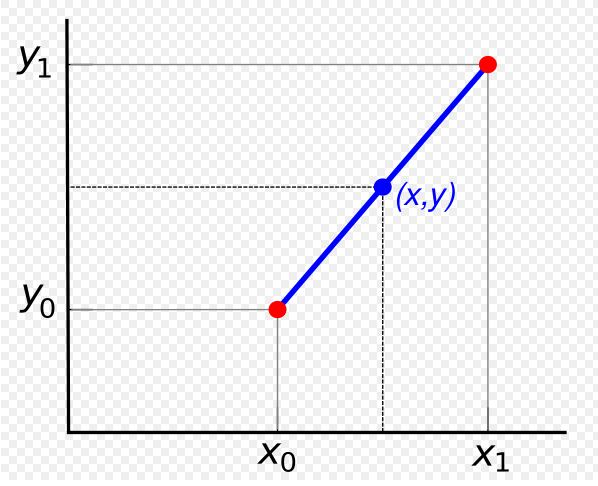
\includegraphics[width=65mm,height=55mm]{p6.JPG}
	\label{fig:p7}
\end{figure}

{\bf Interpolarea unui set de date}\\

Interpolarea unui set de puncte de date $(x_{0},y_{0}),(x_{1},y_{1}),...,(x_{n},y_{n})$ este definit\u{a} ca fiind concatenarea interpol\u{a}rii lineare \^{i}ntre fiecare pereche de puncte a setului de date. Rezultatul va fi o curb\u{a} continu\u{a}, cu o derivat\u{a} discontinu\u{a}, totu\c{s}i de clas\u{a} diferit\u{a} $C^{0}$.

Deseori interpolarea linear\u{a} este folosit\u{a} pentru aproximarea unei valori a  unei func\c{t}ii f folosind dou\u{a} valori cunoscute a acelei func\c{t}ii la fiecare din cele dou\u{a} puncte. Eroarea acestei aproxim\u{a}ri este definit\u{a} ca:
	\[R_{T}=f(x)-p(x)
\]
unde $p$ denot\u{a} interpolarea linear\u{a} polinomial\u{a} definit\u{a} mai jos:
	\[p(x)=f(x_{0})+\frac{f(x_{1})-f(x_{0})}{x_{1}-x_{0}}(x-x_{0})
\]
Se poate defini folosind teorema lui Rolle \footnote{ Studiu aprofundat la: http://en.wikipedia.org/wiki/Rolletheorem } c\u{a} dac\u{a} f are o a doua derivat\u{a} continu\u{a}, eroarea este limitat\u{a} \^{i}n:
	\[|R_{T}|\leq \frac{(x_{1}-x_{0}^{2})}{8}max_{x_{0}\leq x\leq x_{1}}|f^{||}(x)|
\]
Dup\u{a} cum s e vede aproximarea dintre cele dou\u{a} puncte pe o func\c{t}ie definit\u{a} devine din ce \^{i}n ce mai rea cu cea de-a doua derivat\u{a} a func\c{t}iei acre este aproximat\u{a}. 
\begin{figure}
	\centering
		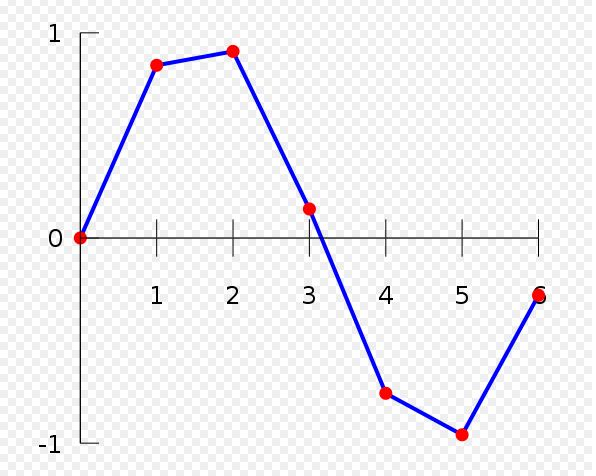
\includegraphics[width=60mm,height=55mm]{p7.JPG}
	\label{fig:p7}
\end{figure}

 

\end{document}